\documentclass[a4paper,portrait]{article}
%\documentclass[border=5mm, 12pt]{standalone}

%\usepackage[latin1]{inputenc}
\usepackage{graphicx}
\usepackage[margin=1.0cm]{geometry}
\usepackage{caption}

\captionsetup{
   justification=raggedright,
   labelfont=bf,
   singlelinecheck=off
}

\renewcommand{\familydefault}{\sfdefault}
\renewcommand{\sfdefault}{phv}

\begin{document}

\begin{figure}[!htbp]%[H]
%\begin{figure}[ht]
\centering
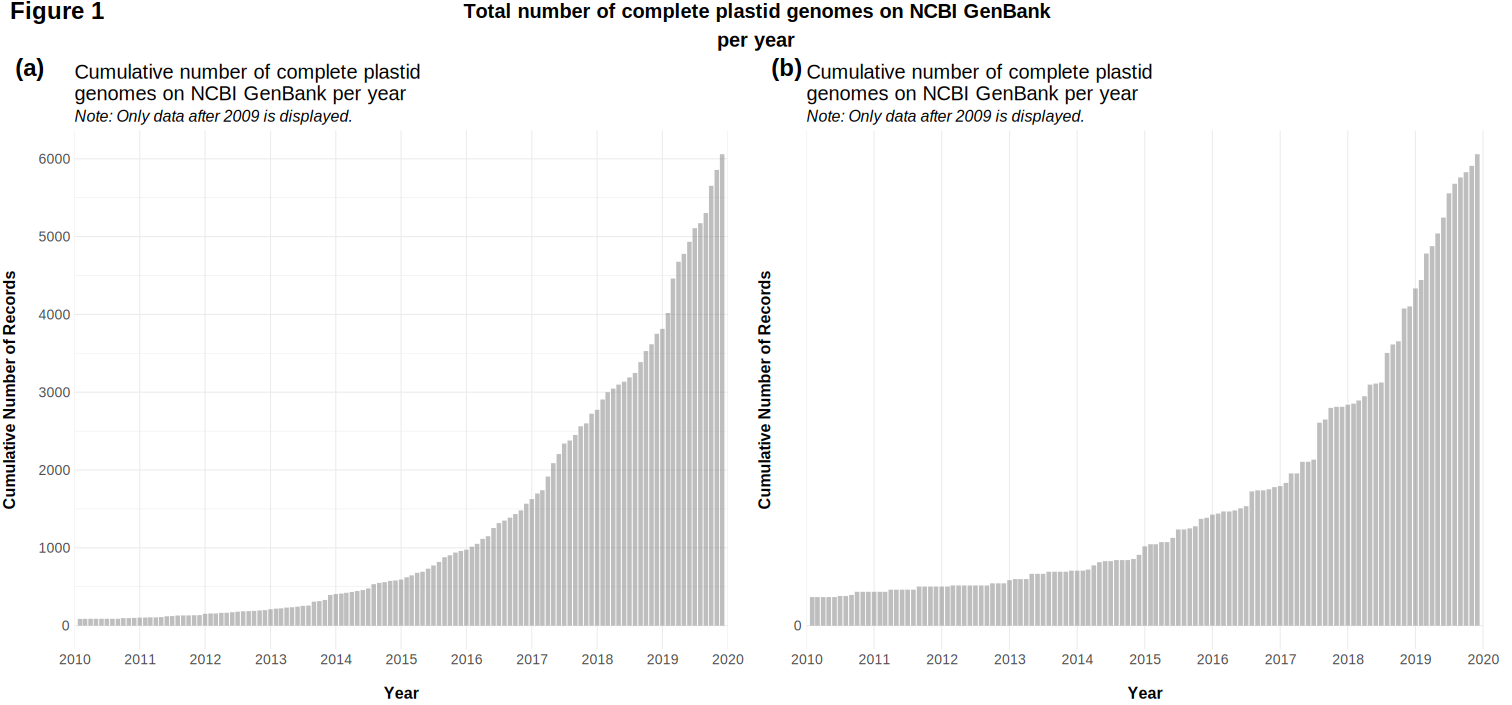
\includegraphics[width=1.00\linewidth]{input/MANUSCRIPT_Figure1.pdf}
\caption{Number of complete plastid genomes of \textbf{(a)} angiosperms and \textbf{(b)} non-angiosperms on NCBI GenBank over the past 10 years (01-Jan-2010 and 31-Dec-2019). The scale of the y-axis is different across plots. All duplicate records generated via the NCBI RefSeq database were excluded prior to plotting.}
\label{fig:Figure1}
\end{figure}

\end{document}
